\documentclass[12pt]{article}
\author{Alex Ho}
\title{FYS4150 - Computational Physics \\ Project 3}
\usepackage{listings}
\usepackage{graphicx}
\usepackage{verbatim}
\usepackage{amsmath}
\usepackage[utf8]{inputenc}
\usepackage{xcolor}
\usepackage{hyperref}

\lstset{
language=Python,
basicstyle=\ttfamily,
otherkeywords={self},             
keywordstyle=\ttfamily\color{blue!90!black},
keywords=[2]{True,False},
%keywords=[3]{ttk},
keywordstyle={[2]\ttfamily\color{blue!90!black}},
emph={MyClass,__init__},          
emphstyle=\ttfamily\color{red!80!black},    
stringstyle=\color{blue!90!black},
showstringspaces=false,
commentstyle=\color{blue!90!black},
breaklines=true,
tabsize=3,
moredelim=**[is][\color{blue}]{@}{@}
}

\begin{document}
\maketitle
\subsection*{3a)}
\subsection*{3b)}
Implementing the Euler and Verlet method is quite easy. We have the Euler method as
\begin{align*}
x_{i+1} = x_i + v_idt \\
v_{i+1} = v_i + a_idt
\end{align*}
One needs to calculate the acceleration $a_i$ using the discretized equations that we have previously shown. One can also implement a more precise method, the Euler Cromer's method, which is given as
\begin{align*}
v_{i+1} = v_i + a_idt \\
x_{i+1} = x_i + v_{i+1}dt
\end{align*}
Which is almost the same as the Euler method, however, the position now depends on the new velocity $v_{i+1}$. Unlike the Euler method, we now need to calculate the new velocity before calculating the new position. In the Euler method, we did not have to take this into account. In the C++ program, the ordering of the position and velocity calculation are swapped for these two methods, and we will see later that this will give two different results.

The next method we will look at is the Verlet method. It is given as
\begin{align*}
x_{i+1} = x_i + v_idt + \frac{dt^2}{2}a_i\\
v_{i+1} = v_i + \frac{dt}{2}\left(a_{i+1} + a_i \right)
\end{align*}
Implementing this may be a little tricky. Calculating the position is straight forward, but the velocity now depends on $a_{i+1}$ and $a_i$. To bypass this problem, we will have to save $a_i$ so its own variable and then calculate the new acceleration $a_{i+1}$ using the new calculated position $x_{i+1}$. 

\subsection*{3c) - Testing algorithm}
The initial velocity of Earth is retrieved by data from NASA.

One can assume that the total energy for the whole system is conserved as the total energy will confined within this system. That is, we think of this system that is in a box. The energy for this system will not leave the box, thus the energy is conserved. We are also not taking into account of gravitational waves, which have some energy as well.

Another way to determine that the energy must be conserved is because the forces in this system are conservative.

%We will now test the Euler and Verlet method, presented earlier, to solve the Earth-Sun system. Figure 1 shows the plots of the Earth-Sun system using Euler (top image) and Verlet method (bottom image). As we can see, the Verlet method gives a more precise and stable Earth orbit, whereas the Euler method gives a less stable Earth orbit.

We will now test the Euler and Verlet method, presented earlier, to solve the Earth-Sun system. We will also see how stable these methods are for different values of $\delta t$. For the C++ program, we have tested $\delta t$ values of 0.0001 and 0.001. The number of mesh points used for each $\delta t$ values is $N = 300 000$ and $N=30 000$ respectively. This is to ensure that the time elapsed, for both simulations, are the same.

Figure 1 shows a comparison of the Euler method with the given $\delta t$ values respectively. The system is a little more stable for a lower $\delta $t value, but Earth seems to go closer and closer to the Sun for every circular orbit. This does not exactly fit with what we observe, so the Euler method is clearly not the most ideal algorithm we can use for these kinds of systems.

Let us now look at the Verlet method. Figure 2 compares the Verlet method of the given $\delta t$ values. As we can see, the system for $\delta t = 0.0001$ is incredibly stable, giving an almost perfect circular orbit for the Earth. The orbit is not perfectly circular is due to very small fluctuations in the orbit of Earth. For a smaller $\delta t$ value, the orbit is still circular, and unlike the Euler method, Earth will not fall towards the Sun. However, the fluctuations now are a little bigger, which is why the circular line in figure 2 is a little bit thicker. 

%  As we can see, lower values of $\delta t$ gives a more stable system. However, even though the system is more stable, the orbit of Earth seems to differ quite significantly for each 

For the C++ program, the time difference between these two methods are almost negligible for a small number of time steps. The Verlet method had to run roughly 2 times longer compared to the Euler method, which is not surprising due to the increased number of FLOPS required to solve one time step. However, as we saw from the plots, the extra time it took for the Verlet method gave a much better result than the one using Euler method.

\begin{lstlisting}
@Running Euler method
Time elapsed for Euler method:0.1s
Data saved to: Earth_Sun_sys_euler.txt

Running Euler Cromer method
Time elapsed for Euler Cromer method:0.097s
Data saved to: Earth_Sun_sys_eulercromer.txt

Running Verlet method
Time elapsed for Verlet method:0.202s
Data saved to: Earth_Sun_sys_verlet.txt@
\end{lstlisting}

One can also use the Euler Cromer method to solve these systems. A plot of the Earth-Sun system using the Euler Cromer method can be found in the appendix. As we can see, the results practically identical to the Verlet method. The computation speed of the Euler Cromer method is practically the same as Euler method.

\begin{figure}[hbtp]
\centering
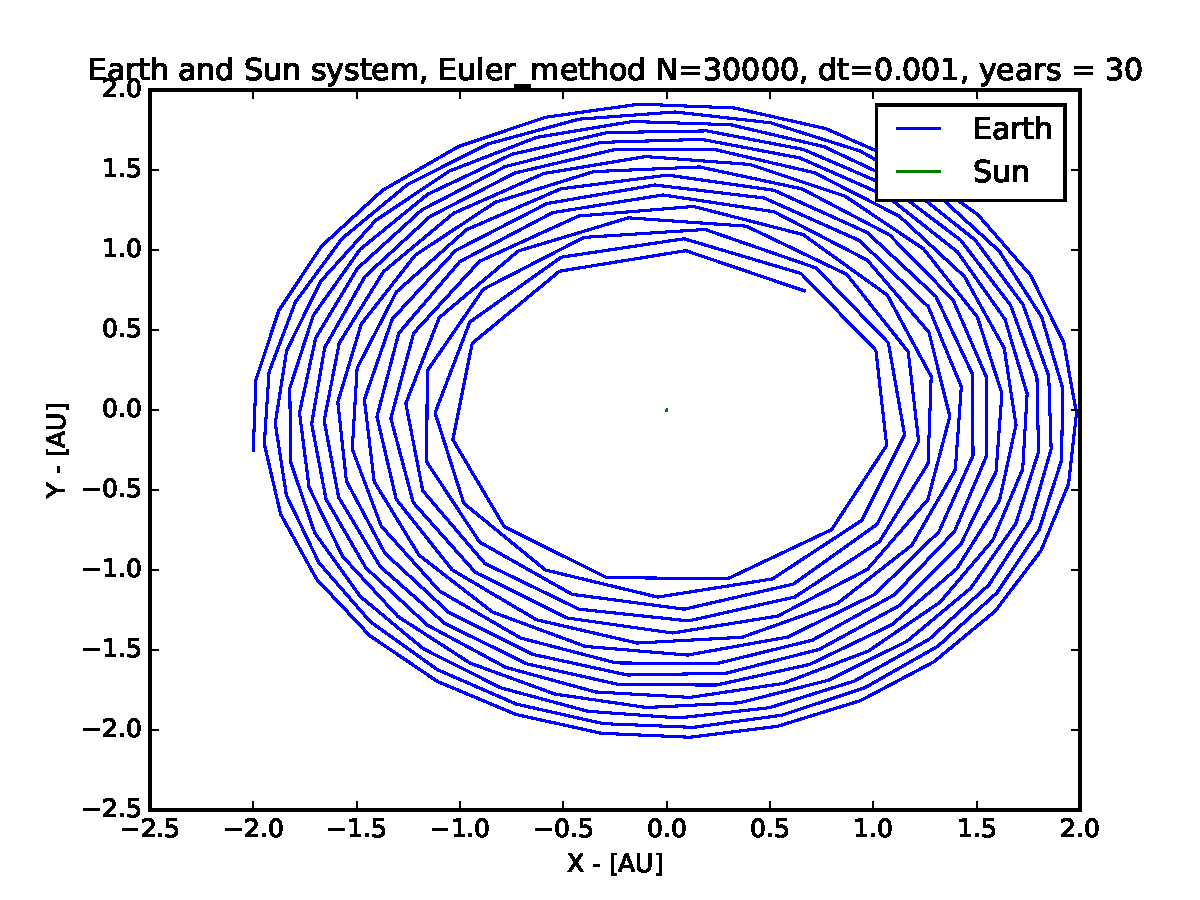
\includegraphics[width=\linewidth]{Plots/Earth_Sun_Euler_method.pdf}
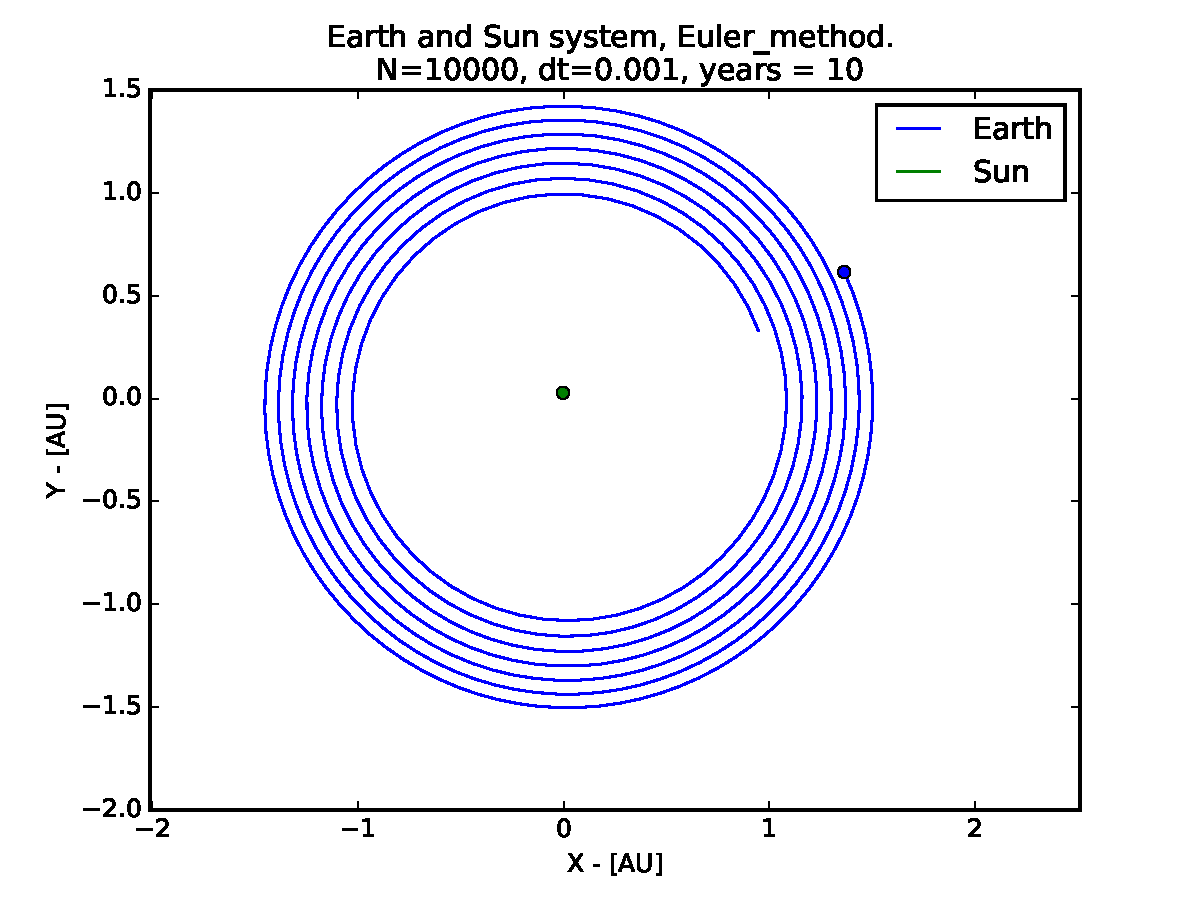
\includegraphics[width=\linewidth]{Plots/Earth_Sun_Euler_method_larger_dt.pdf} 
\caption{Euler method comparison for different $\delta t$}
\end{figure}

\begin{figure}[hbtp]
\centering
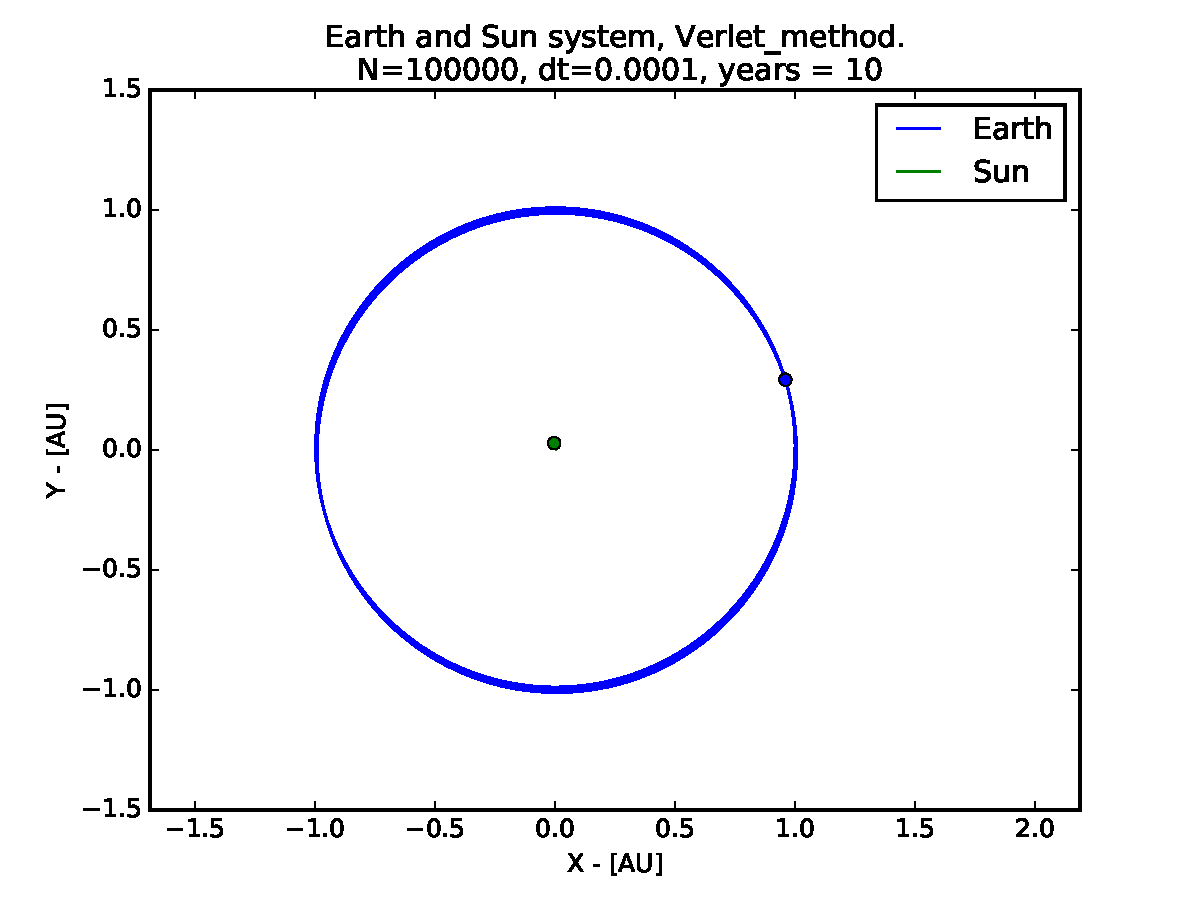
\includegraphics[width=\linewidth]{Plots/Earth_Sun_Verlet_method.pdf}
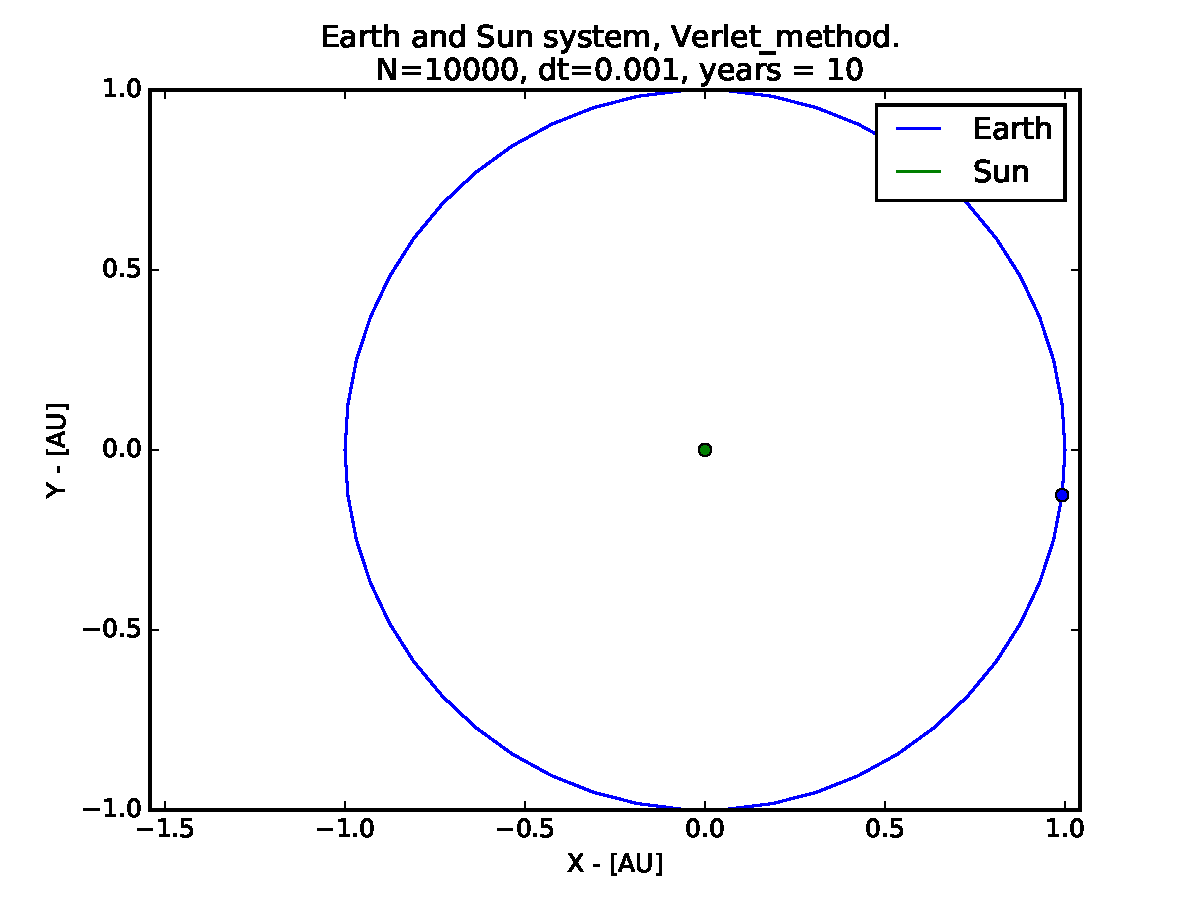
\includegraphics[width=\linewidth]{Plots/Earth_Sun_Verlet_method_larger_dt.pdf}
\caption{Verlet method comparison for different $\delta t$}
\end{figure}

\newpage
\subsection*{3d) - Escape velocity}
One can calculate the escape velocity of a planet analytically. The escape velocity of an object with mass $M_1$ is the velocity when the object's kinetic energy is equal to the potential energy. That is
\begin{align*}
\frac{1}{2}M_1v = \frac{GM_1M_2}{r}
\end{align*}
Let us consider a planet with mass $M$ orbiting around the Sun. The escape velocity for this planet is then
\begin{align*}
v_{escape} = \sqrt{\frac{2GM_{\odot}}{r}}
\end{align*}
In terms of AU per year, we have that $GM_{\odot} = 4\pi^2 \text{AU}^3/\text{yr}^2$, so
\begin{align*}
v_{escape} = \sqrt{\frac{8\pi^2}{r}} \text{AU}/\text{yr}
\end{align*}
It is now quite easy to implement the escape velocity. In the C++ program, we have assumed that the planet has the mass of Earth and start 1 AU away from the Sun in the x direction. The velocity will be the escape velocity directed in the y-direction. 

\begin{figure}[hbtp]
\centering
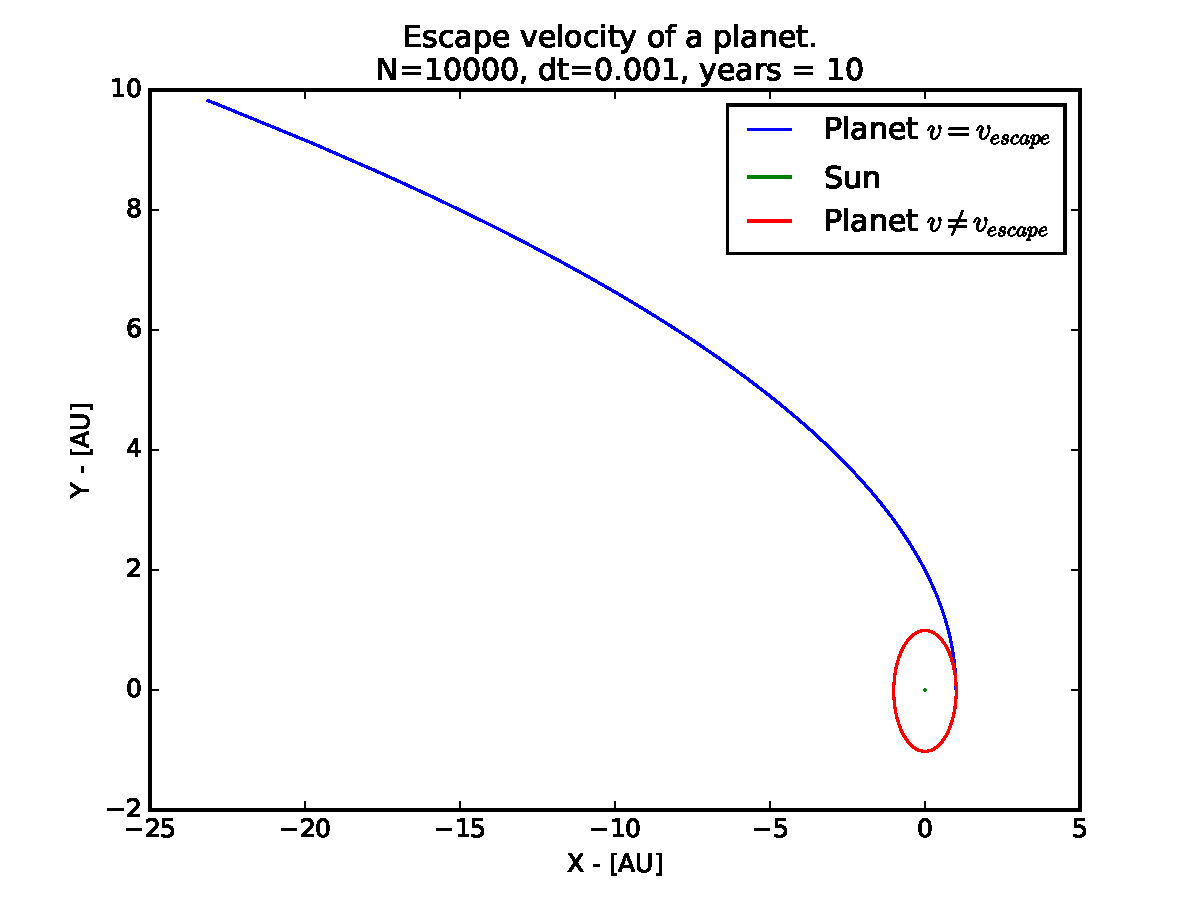
\includegraphics[width=\linewidth]{Plots/Escape_velocity.pdf}
\caption{Plot shows a planet with the mass of Earth with and without escape velocity.}
\end{figure}


\newpage 
\subsection*{3e) - Three body problem}
We already know that Earth's orbit will change a little bit when we add Jupiter to the system. Figure 3 shows the orbit of the Earth and Jupiter, as well as the Sun. The orbits themselves does not look particularly odd in any way, but it is hard to see how Jupiter affects the orbit of the Earth. Instead, we only plot the orbit of the Earth and the Sun (still taking Jupiter into account during the calculations) which can be found in figure 4. 

As we can see from figure 4, the orbit of the Earth has changed quite a bit compared to the system without Jupiter. Before we added Jupiter into the system, Earth's orbit was circular. Now that we have added Jupiter into the system, Earth's orbit is now ecliptic, which is a little bit more realistic if we compare it to the orbit we observe. In addition to that, the position of the Sun is also affected a little bit. The Sun is no longer at rest, which means that the Sun is not the center of mass in the system.

A 3D plot of this system can be found in the appendix.

\begin{figure}[hbtp]
\centering\textbf{•}
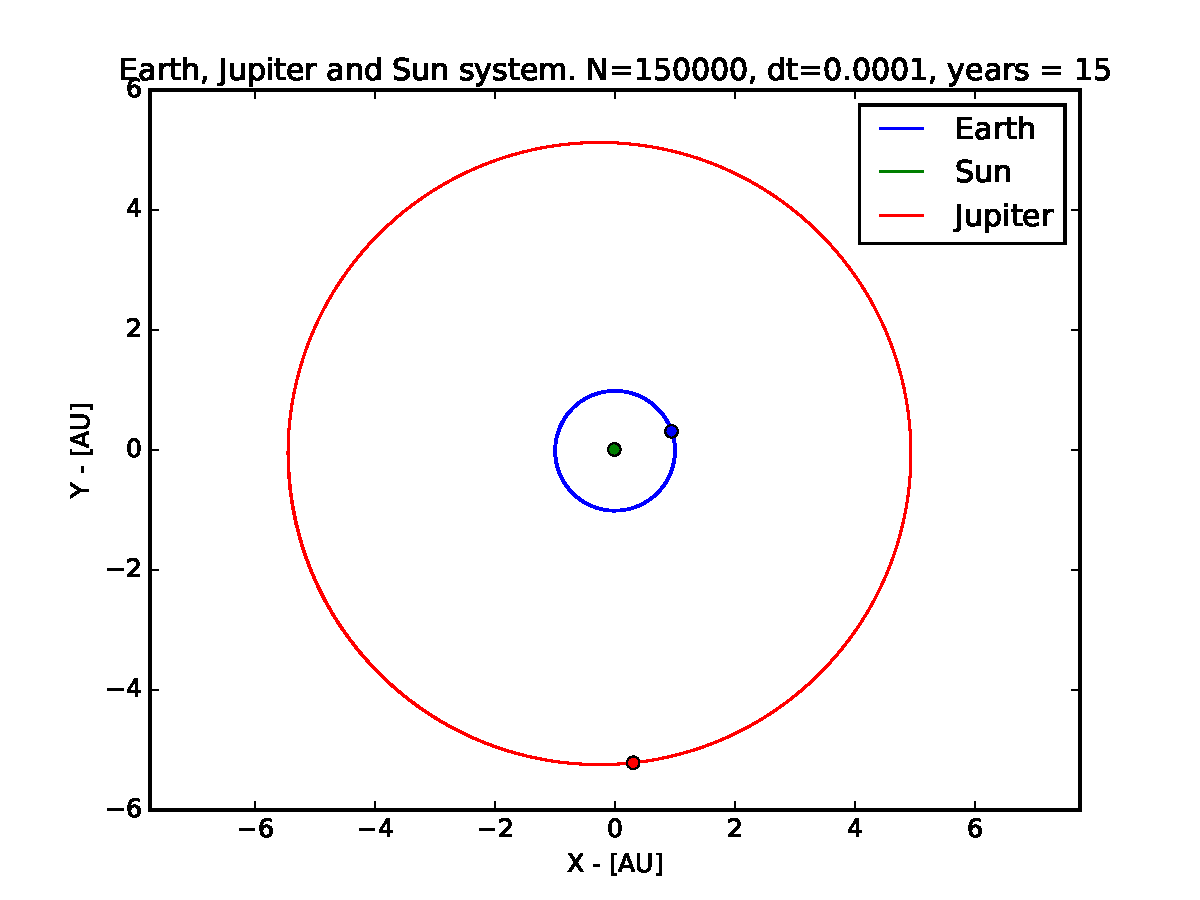
\includegraphics[width=\linewidth]{Plots/Earth_Sun_Jupiter.pdf}
\caption{Orbits of the Earth, Jupiter and the Sun.}
\end{figure}

\begin{figure}[hbtp]
\centering
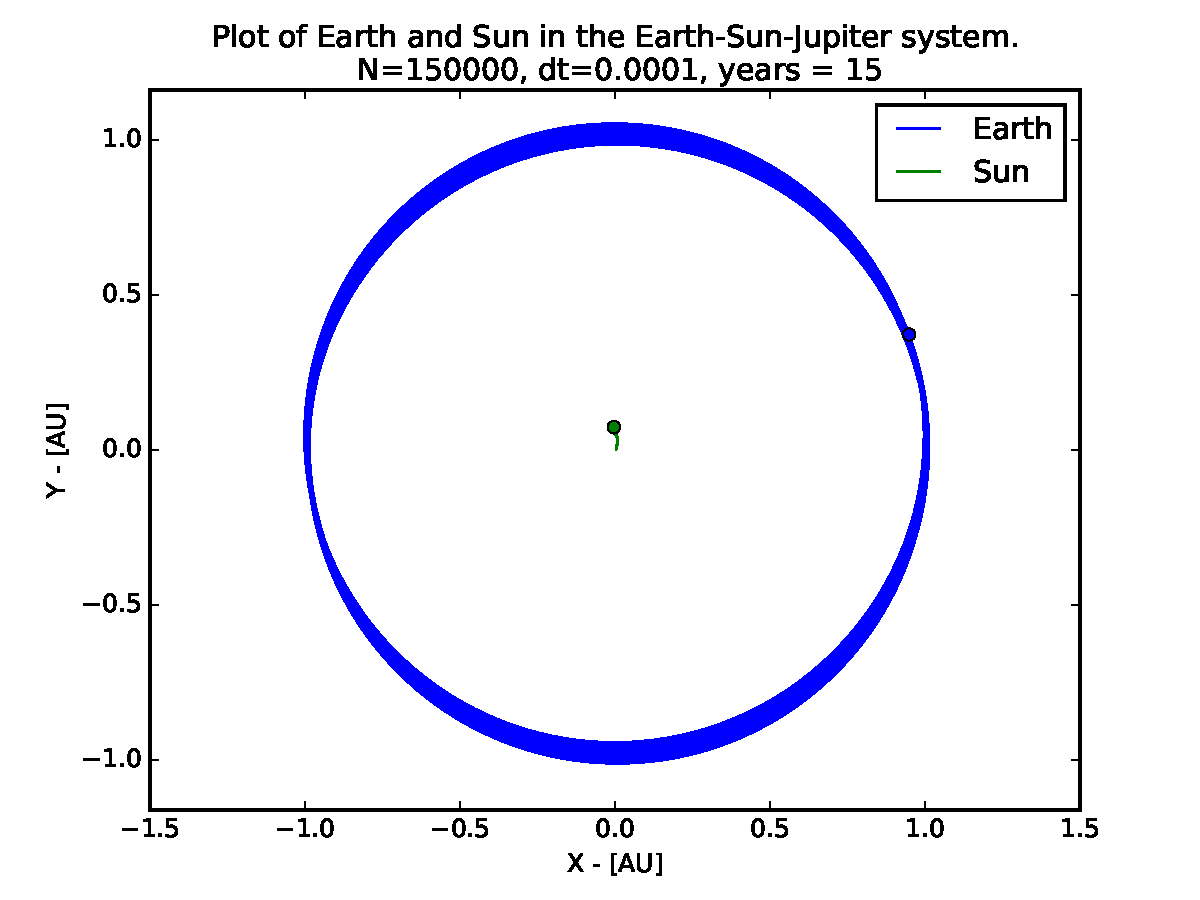
\includegraphics[width=\linewidth]{Plots/ESJ_EarthandSun.pdf}
\caption{Plot of the Earth and the Sun in the Earth-Sun-Jupiter system.}
\end{figure}

\newpage

\subsection*{3f)}
We will now add all planets, including Pluto, into our system. This is quite straight forward to do. In the C++ program, all we have to do is to add an extra force to each planet. Figure 4 shows the orbits of all planets in 3 dimensions. Because of the orbit sizes of the outer planets (i.e Jupiter, Saturn, Uranus, Neptune and Pluto), the orbits of the first four planets will be packed in the center of the system, which is quite hard to analyse. 

What we can do, is to reduce the value of $\delta t$ to simulate the first four planets, while still taking the effect of the gravitational forces of the other planets into account. This will of course reduce the number of years the simulation shows, which means that the outer planets will not have full orbits.

\begin{figure}[hbtp]
\centering
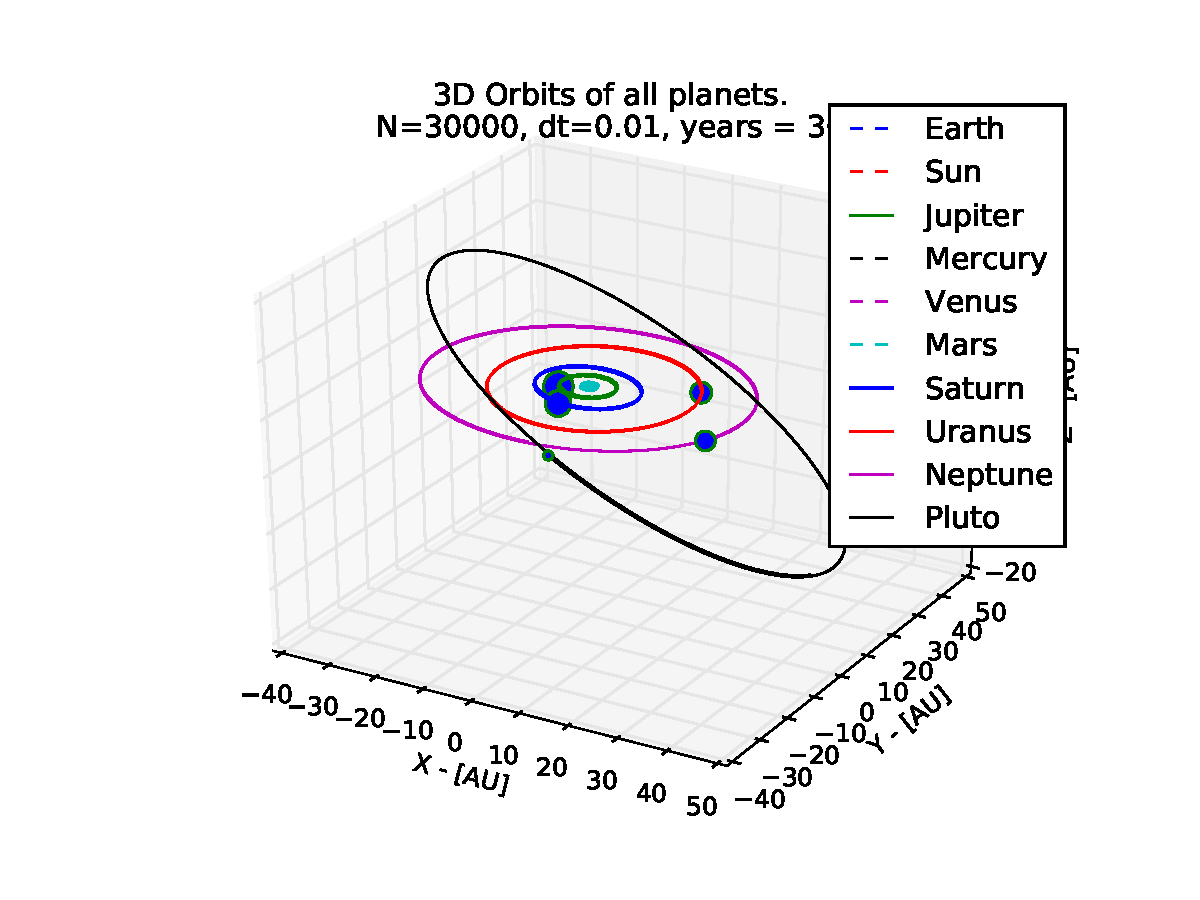
\includegraphics[width=\linewidth]{Plots/All_planets_3D_plot.pdf}
\caption{Plot of all planets in 3D. Note: the scatter plot (spheres) of the planet does not scale with it's real size.}
\end{figure}
\begin{figure}[hbtp]
\centering
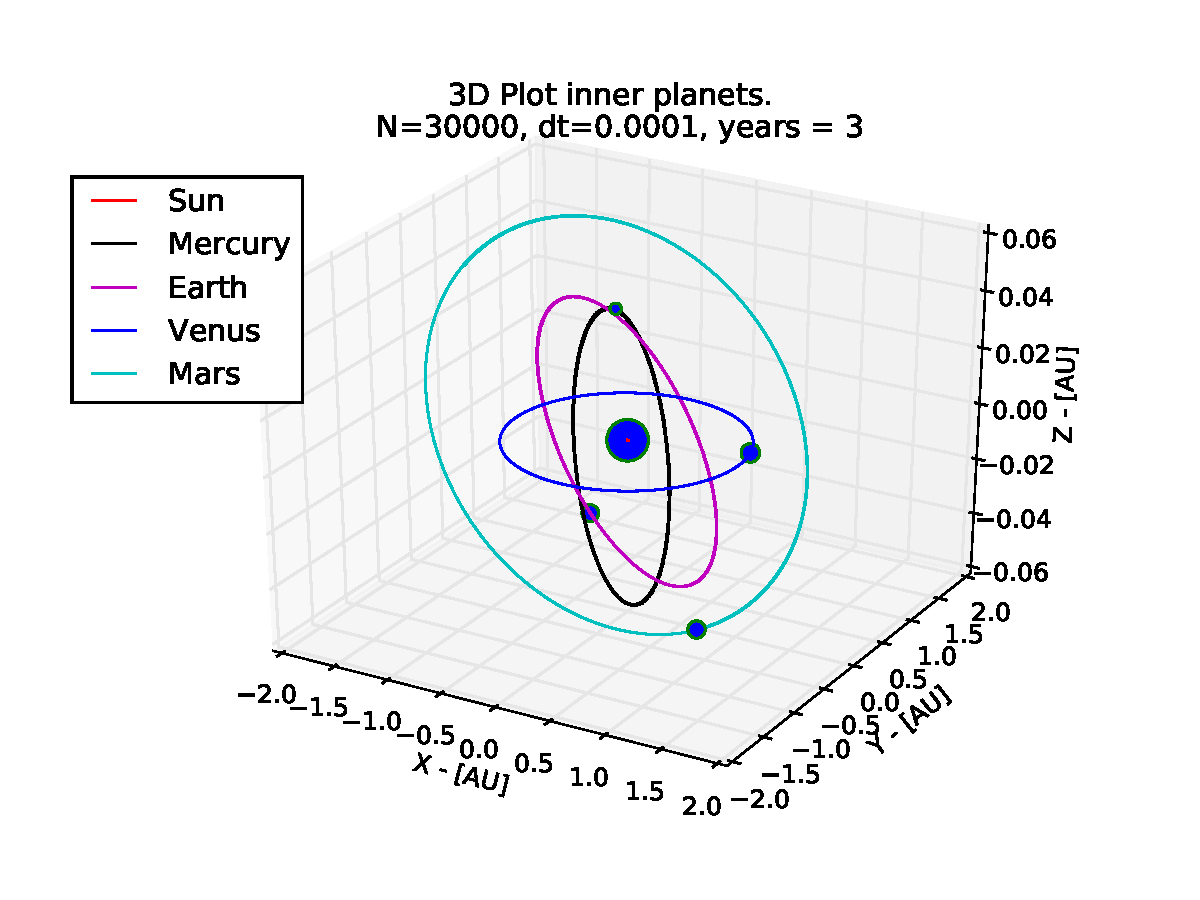
\includegraphics[width=\linewidth]{Plots/First_planets_3D_plot.pdf}
\caption{3D plot of the first four planets orbit. Note: the scatter plot (spheres) of the planet does not scale with it's real size.}
\end{figure}

\newpage
\section*{Appendix}
\begin{figure}[hbtp]
\centering
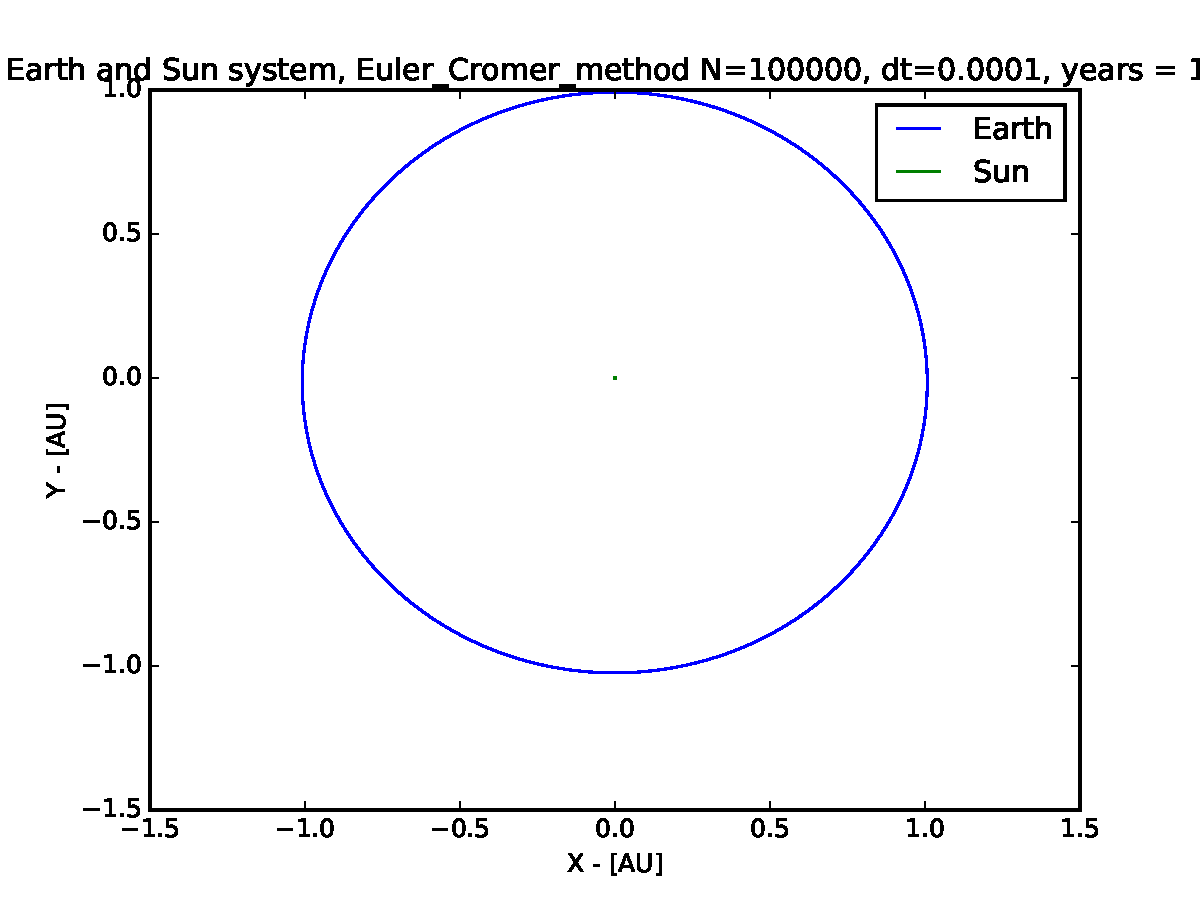
\includegraphics[width=\linewidth]{Plots/Earth_Sun_Euler_Cromer_method.pdf}
\caption{Earth-Sun system using Euler Cromer method}
\end{figure}

\begin{figure}[hbtp]
\centering
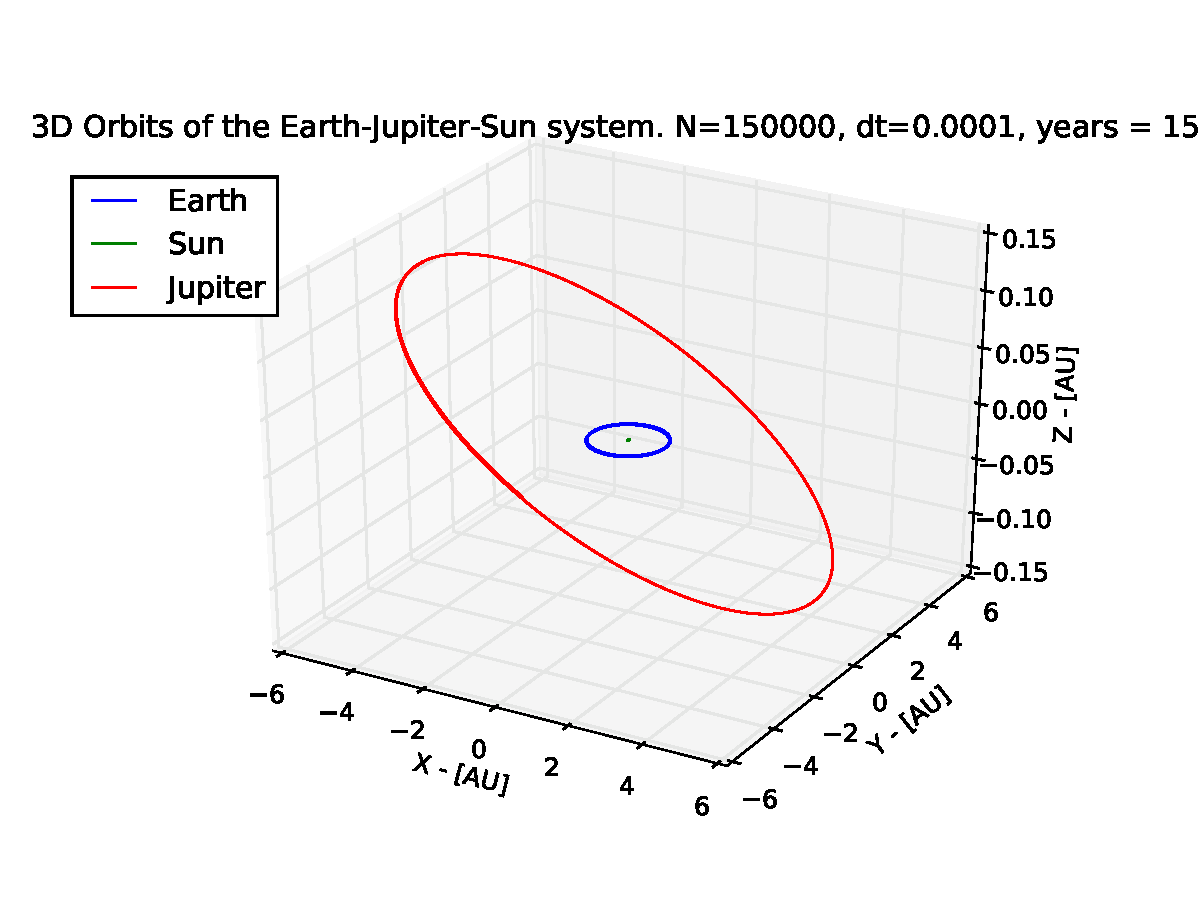
\includegraphics[width=\linewidth]{Plots/Earth_Sun_Jupiter_3D.pdf}
\caption{3D Plot of the Earth-Sun-Jupiter system.}
\end{figure}


\end{document}